\documentclass[11pt,a4paper]{article}

\usepackage[margin=1in]{geometry}
\usepackage{graphicx}
\usepackage{booktabs}
\usepackage{hyperref}
\usepackage{amsmath}
\usepackage{xcolor}
\usepackage{float}
\usepackage{subcaption}
\usepackage{enumitem}

\newcommand{\todo}[1]{{\color{red}\textbf{[TODO: #1]}}}

% Auto-generated data macros from benchmark results.
% Regenerate: cd task2 && python3 generate_data.py
% AUTO-GENERATED by generate_data.py -- do not edit by hand
% Re-run:  cd task2 && python3 generate_data.py


% === SIMD width speedups, GFLOP/s, instruction counts ===
\newcommand{\simdWidthNaiveOhtwentyeightGflops}{3.33}
\newcommand{\simdWidthNaiveOhtwentyeightSpeedup}{1.00x}
\newcommand{\simdWidthNaiveOhtwentyeightInsns}{94,691,884}
\newcommand{\simdWidthSSEOhtwentyeightGflops}{46.48}
\newcommand{\simdWidthSSEOhtwentyeightSpeedup}{13.94x}
\newcommand{\simdWidthSSEOhtwentyeightInsns}{101,691,574}
\newcommand{\simdWidthAVXOhtwentyeightGflops}{89.68}
\newcommand{\simdWidthAVXOhtwentyeightSpeedup}{26.90x}
\newcommand{\simdWidthAVXOhtwentyeightInsns}{99,048,350}
\newcommand{\simdWidthAVXFiveTwelveOhtwentyeightGflops}{89.46}
\newcommand{\simdWidthAVXFiveTwelveOhtwentyeightSpeedup}{26.84x}
\newcommand{\simdWidthAVXFiveTwelveOhtwentyeightInsns}{97,792,306}
\newcommand{\simdWidthNaiveTwofiftysixGflops}{2.64}
\newcommand{\simdWidthNaiveTwofiftysixSpeedup}{1.00x}
\newcommand{\simdWidthNaiveTwofiftysixInsns}{721,951,242}
\newcommand{\simdWidthSSETwofiftysixGflops}{50.75}
\newcommand{\simdWidthSSETwofiftysixSpeedup}{19.20x}
\newcommand{\simdWidthSSETwofiftysixInsns}{773,677,911}
\newcommand{\simdWidthAVXTwofiftysixGflops}{87.95}
\newcommand{\simdWidthAVXTwofiftysixSpeedup}{33.27x}
\newcommand{\simdWidthAVXTwofiftysixInsns}{751,129,706}
\newcommand{\simdWidthAVXFiveTwelveTwofiftysixGflops}{108.57}
\newcommand{\simdWidthAVXFiveTwelveTwofiftysixSpeedup}{41.07x}
\newcommand{\simdWidthAVXFiveTwelveTwofiftysixInsns}{740,383,994}
\newcommand{\simdWidthNaiveFtwelveGflops}{2.41}
\newcommand{\simdWidthNaiveFtwelveSpeedup}{1.00x}
\newcommand{\simdWidthNaiveFtwelveInsns}{5,700,178,491}
\newcommand{\simdWidthSSEFtwelveGflops}{51.34}
\newcommand{\simdWidthSSEFtwelveSpeedup}{21.28x}
\newcommand{\simdWidthSSEFtwelveInsns}{6,098,319,894}
\newcommand{\simdWidthAVXFtwelveGflops}{90.90}
\newcommand{\simdWidthAVXFtwelveSpeedup}{37.67x}
\newcommand{\simdWidthAVXFtwelveInsns}{5,912,668,975}
\newcommand{\simdWidthAVXFiveTwelveFtwelveGflops}{112.14}
\newcommand{\simdWidthAVXFiveTwelveFtwelveSpeedup}{46.47x}
\newcommand{\simdWidthAVXFiveTwelveFtwelveInsns}{5,821,928,574}
\newcommand{\simdWidthNaiveTtwentyfourGflops}{2.30}
\newcommand{\simdWidthNaiveTtwentyfourSpeedup}{1.00x}
\newcommand{\simdWidthNaiveTtwentyfourInsns}{45,378,549,503}
\newcommand{\simdWidthSSETtwentyfourGflops}{50.52}
\newcommand{\simdWidthSSETtwentyfourSpeedup}{22.00x}
\newcommand{\simdWidthSSETtwentyfourInsns}{48,498,010,433}
\newcommand{\simdWidthAVXTtwentyfourGflops}{82.41}
\newcommand{\simdWidthAVXTtwentyfourSpeedup}{35.89x}
\newcommand{\simdWidthAVXTtwentyfourInsns}{46,990,364,336}
\newcommand{\simdWidthAVXFiveTwelveTtwentyfourGflops}{99.28}
\newcommand{\simdWidthAVXFiveTwelveTtwentyfourSpeedup}{43.24x}
\newcommand{\simdWidthAVXFiveTwelveTtwentyfourInsns}{46,246,355,457}
\newcommand{\simdWidthNaiveTfortyeightGflops}{2.21}
\newcommand{\simdWidthNaiveTfortyeightSpeedup}{1.00x}
\newcommand{\simdWidthNaiveTfortyeightInsns}{362,206,124,379}
\newcommand{\simdWidthSSETfortyeightGflops}{35.68}
\newcommand{\simdWidthSSETfortyeightSpeedup}{16.13x}
\newcommand{\simdWidthSSETfortyeightInsns}{386,920,963,092}
\newcommand{\simdWidthAVXTfortyeightGflops}{46.18}
\newcommand{\simdWidthAVXTfortyeightSpeedup}{20.87x}
\newcommand{\simdWidthAVXTfortyeightInsns}{374,781,905,812}
\newcommand{\simdWidthAVXFiveTwelveTfortyeightGflops}{52.09}
\newcommand{\simdWidthAVXFiveTwelveTfortyeightSpeedup}{23.54x}
\newcommand{\simdWidthAVXFiveTwelveTfortyeightInsns}{368,749,447,552}

% === Size sweep: simd / prefetch / optimized ===
\newcommand{\sweepSimdOhtwentyeightNaiveGflops}{2.81}
\newcommand{\sweepSimdOhtwentyeightGflops}{84.00}
\newcommand{\sweepSimdOhtwentyeightSpeedup}{29.91x}
\newcommand{\sweepPrefetchOhtwentyeightNaiveGflops}{2.76}
\newcommand{\sweepPrefetchOhtwentyeightGflops}{54.42}
\newcommand{\sweepPrefetchOhtwentyeightSpeedup}{19.71x}
\newcommand{\sweepOptimizedOhtwentyeightNaiveGflops}{2.72}
\newcommand{\sweepOptimizedOhtwentyeightGflops}{56.88}
\newcommand{\sweepOptimizedOhtwentyeightSpeedup}{20.95x}
\newcommand{\sweepSimdTwofiftysixNaiveGflops}{2.38}
\newcommand{\sweepSimdTwofiftysixGflops}{85.04}
\newcommand{\sweepSimdTwofiftysixSpeedup}{35.77x}
\newcommand{\sweepPrefetchTwofiftysixNaiveGflops}{2.40}
\newcommand{\sweepPrefetchTwofiftysixGflops}{48.06}
\newcommand{\sweepPrefetchTwofiftysixSpeedup}{20.00x}
\newcommand{\sweepOptimizedTwofiftysixNaiveGflops}{2.43}
\newcommand{\sweepOptimizedTwofiftysixGflops}{58.68}
\newcommand{\sweepOptimizedTwofiftysixSpeedup}{24.14x}
\newcommand{\sweepSimdThreeeightyfourNaiveGflops}{2.34}
\newcommand{\sweepSimdThreeeightyfourGflops}{88.46}
\newcommand{\sweepSimdThreeeightyfourSpeedup}{37.76x}
\newcommand{\sweepPrefetchThreeeightyfourNaiveGflops}{2.34}
\newcommand{\sweepPrefetchThreeeightyfourGflops}{54.05}
\newcommand{\sweepPrefetchThreeeightyfourSpeedup}{23.11x}
\newcommand{\sweepOptimizedThreeeightyfourNaiveGflops}{2.33}
\newcommand{\sweepOptimizedThreeeightyfourGflops}{63.42}
\newcommand{\sweepOptimizedThreeeightyfourSpeedup}{27.18x}
\newcommand{\sweepSimdFtwelveNaiveGflops}{2.30}
\newcommand{\sweepSimdFtwelveGflops}{87.15}
\newcommand{\sweepSimdFtwelveSpeedup}{37.93x}
\newcommand{\sweepPrefetchFtwelveNaiveGflops}{2.29}
\newcommand{\sweepPrefetchFtwelveGflops}{56.97}
\newcommand{\sweepPrefetchFtwelveSpeedup}{24.87x}
\newcommand{\sweepOptimizedFtwelveNaiveGflops}{2.31}
\newcommand{\sweepOptimizedFtwelveGflops}{65.22}
\newcommand{\sweepOptimizedFtwelveSpeedup}{28.20x}
\newcommand{\sweepSimdSevensixtyeightNaiveGflops}{2.21}
\newcommand{\sweepSimdSevensixtyeightGflops}{76.58}
\newcommand{\sweepSimdSevensixtyeightSpeedup}{34.66x}
\newcommand{\sweepPrefetchSevensixtyeightNaiveGflops}{2.21}
\newcommand{\sweepPrefetchSevensixtyeightGflops}{54.37}
\newcommand{\sweepPrefetchSevensixtyeightSpeedup}{24.57x}
\newcommand{\sweepOptimizedSevensixtyeightNaiveGflops}{2.23}
\newcommand{\sweepOptimizedSevensixtyeightGflops}{62.48}
\newcommand{\sweepOptimizedSevensixtyeightSpeedup}{28.04x}
\newcommand{\sweepSimdTtwentyfourNaiveGflops}{2.19}
\newcommand{\sweepSimdTtwentyfourGflops}{77.16}
\newcommand{\sweepSimdTtwentyfourSpeedup}{35.18x}
\newcommand{\sweepPrefetchTtwentyfourNaiveGflops}{2.17}
\newcommand{\sweepPrefetchTtwentyfourGflops}{54.06}
\newcommand{\sweepPrefetchTtwentyfourSpeedup}{24.93x}
\newcommand{\sweepOptimizedTtwentyfourNaiveGflops}{2.15}
\newcommand{\sweepOptimizedTtwentyfourGflops}{62.56}
\newcommand{\sweepOptimizedTtwentyfourSpeedup}{29.07x}
\newcommand{\sweepSimdFifteenthirtysixNaiveGflops}{2.08}
\newcommand{\sweepSimdFifteenthirtysixGflops}{36.77}
\newcommand{\sweepSimdFifteenthirtysixSpeedup}{17.69x}
\newcommand{\sweepPrefetchFifteenthirtysixNaiveGflops}{2.10}
\newcommand{\sweepPrefetchFifteenthirtysixGflops}{55.05}
\newcommand{\sweepPrefetchFifteenthirtysixSpeedup}{26.20x}
\newcommand{\sweepOptimizedFifteenthirtysixNaiveGflops}{2.10}
\newcommand{\sweepOptimizedFifteenthirtysixGflops}{63.31}
\newcommand{\sweepOptimizedFifteenthirtysixSpeedup}{30.15x}
\newcommand{\sweepSimdTfortyeightNaiveGflops}{2.06}
\newcommand{\sweepSimdTfortyeightGflops}{44.91}
\newcommand{\sweepSimdTfortyeightSpeedup}{21.82x}
\newcommand{\sweepPrefetchTfortyeightNaiveGflops}{2.19}
\newcommand{\sweepPrefetchTfortyeightGflops}{55.25}
\newcommand{\sweepPrefetchTfortyeightSpeedup}{25.21x}
\newcommand{\sweepOptimizedTfortyeightNaiveGflops}{2.20}
\newcommand{\sweepOptimizedTfortyeightGflops}{63.96}
\newcommand{\sweepOptimizedTfortyeightSpeedup}{29.10x}

% === Perf counters (M=N=K=1024, cold cache) ===
\newcommand{\perfNaiveInsns}{6,452,951,452}
\newcommand{\perfNaiveLoneDmiss}{67,218,496}
\newcommand{\perfNaiveLtwoMiss}{67,567,994}
\newcommand{\perfNaiveLLCmiss}{12,599}
\newcommand{\perfNaiveIPC}{1.52}
\newcommand{\perfSimdInsns}{228,860,073}
\newcommand{\perfSimdLoneDmiss}{17,077,579}
\newcommand{\perfSimdLtwoMiss}{17,105,429}
\newcommand{\perfSimdLLCmiss}{33,959}
\newcommand{\perfSimdIPC}{2.01}
\newcommand{\perfPrefetchInsns}{330,758,988}
\newcommand{\perfPrefetchLoneDmiss}{35,317,236}
\newcommand{\perfPrefetchLtwoMiss}{1,315,980}
\newcommand{\perfPrefetchLLCmiss}{12,910}
\newcommand{\perfPrefetchIPC}{1.98}
\newcommand{\perfOptimizedInsns}{317,024,417}
\newcommand{\perfOptimizedLoneDmiss}{35,366,614}
\newcommand{\perfOptimizedLtwoMiss}{1,308,706}
\newcommand{\perfOptimizedLLCmiss}{14,109}
\newcommand{\perfOptimizedIPC}{2.19}



\title{CS683 Programming Assignment 1 --- Task 2\\
Matrix Multiplication for Inference}
\author{Avinash Chaudhari -- 23B1064 \and Pranay Marumamula -- 23B1073 \and Siddhant Mulkikar -- 23B0956 \and Madhav R Babu -- 23B1060}
\date{Autumn 2026}

\begin{document}
\maketitle

% ============================================================================
\section{System Configuration}
% ============================================================================

\begin{itemize}
    \item \textbf{CPU:} Intel Core i5-11400H (Tiger Lake-H), 6 cores / 6 threads
          (SMT disabled), all identical P-cores, base 2.70 GHz, max 4.50 GHz
    \item \textbf{L1-D Cache:} 48 KiB per core (288 KiB total, 6 instances),
          64-byte lines, 12-way set associative
    \item \textbf{L2 Cache:} 1.25 MiB per core (7.5 MiB total, 6 instances), 20-way
    \item \textbf{L3 Cache:} 12 MiB (1 instance, shared), 8-way
    \item \textbf{Vector ISA:} AVX2 + FMA and AVX-512
          (\texttt{avx512f}, \texttt{avx512dq}, \texttt{avx512bw}, \texttt{avx512vl},
          \texttt{avx512\_vnni})
    \item \textbf{Compiler flags:} \texttt{-std=c++17 -O2 -fno-tree-vectorize -mavx2 -mfma}
    \item \textbf{OS:} Ubuntu 24.04.4 LTS, kernel 6.8.0-138-generic (x86\_64)
    \item \textbf{Pinning:} \texttt{taskset -c 3}. This CPU is not hybrid, so every core
          is equivalent; a single fixed core is used so all measurements share one
          cache and frequency context.
    \item \textbf{Frequency governor:} \texttt{performance}, with
          \texttt{kernel.perf\_event\_paranoid = -1} so \texttt{perf} can read the
          hardware counters used for cache miss and instruction count measurements.
\end{itemize}

% ============================================================================
\section{Task 2A: Software Prefetching (5 points)}
% ============================================================================

\todo{Task 2A to be completed separately.}

% ============================================================================
\section{Task 2B: SIMD (1 point)}
% ============================================================================

\subsection{SIMD Implementation}

The SGEMM kernel uses a \textbf{register-tiled vectorized dot product} approach.
The matrix layout stores both $A$ and $B$ with the reduction axis $K$ as the contiguous (unit-stride) dimension: $C[i][j] = \sum_p A[i][p] \cdot B[j][p]$.
This means the natural SIMD strategy is to vectorize the dot product over $p$.

The micro-kernel computes a $4 \times 2$ block of $C$ at once using 8 independent \texttt{\_\_m256} accumulators:
\begin{itemize}[nosep]
    \item For each step along $K$, two \texttt{\_mm256\_loadu\_ps} loads fetch 8 elements from two rows of $B$.
    \item Four \texttt{\_mm256\_broadcast\_ss} calls broadcast one element from each of four $A$ rows.
    \item Eight \texttt{\_mm256\_fmadd\_ps} instructions accumulate all $4 \times 2 = 8$ partial-product vectors.
\end{itemize}
This yields 8 FMAs per step from only 6 loads, and the 8 independent accumulator chains saturate the FMA pipeline (FMA latency ${\sim}4$ cycles, throughput $2$/cycle, requiring ${\geq}8$ independent chains).
After the $K$ loop, each accumulator is horizontally reduced (\texttt{hsum256}) to a single scalar, stored into the corresponding $C[i][j]$.

Leftover rows ($M \bmod 4$), columns ($N \bmod 2$), and $K$ elements ($K \bmod 8$) fall to a scalar cleanup path.

Three SIMD widths were benchmarked:
\begin{itemize}[nosep]
    \item \textbf{SSE 128-bit}: 4 floats per vector, $4 \times 2$ register tile, 8 accumulators
    \item \textbf{AVX2 256-bit}: 8 floats per vector, $4 \times 2$ register tile, 8 accumulators
    \item \textbf{AVX-512 512-bit}: 16 floats per vector, $4 \times 2$ register tile, 8 accumulators
\end{itemize}
None of these include cache blocking --- the kernel streams through $A$ and $B$ from whatever cache level holds them.

\subsection{Instruction Count and Performance}

\begin{table}[H]
\centering
\caption{Instruction count and speedup for different SIMD widths}
\resizebox{\textwidth}{!}{%
\begin{tabular}{ll|rrrrr}
\toprule
& & \multicolumn{5}{c}{Matrix Size ($M = N = K$)} \\
Metrics & & 128 & 256 & 512 & 1024 & 2048 \\
\midrule
\textbf{No SIMD}  & Instructions & \simdWidthNaiveOhtwentyeightInsns & \simdWidthNaiveTwofiftysixInsns & \simdWidthNaiveFtwelveInsns & \simdWidthNaiveTtwentyfourInsns & \simdWidthNaiveTfortyeightInsns \\
                   & GFLOP/s      & \simdWidthNaiveOhtwentyeightGflops & \simdWidthNaiveTwofiftysixGflops & \simdWidthNaiveFtwelveGflops & \simdWidthNaiveTtwentyfourGflops & \simdWidthNaiveTfortyeightGflops \\
\midrule
\textbf{SSE 128}   & Instructions & \simdWidthSSEOhtwentyeightInsns & \simdWidthSSETwofiftysixInsns & \simdWidthSSEFtwelveInsns & \simdWidthSSETtwentyfourInsns & \simdWidthSSETfortyeightInsns \\
                   & GFLOP/s      & \simdWidthSSEOhtwentyeightGflops & \simdWidthSSETwofiftysixGflops & \simdWidthSSEFtwelveGflops & \simdWidthSSETtwentyfourGflops & \simdWidthSSETfortyeightGflops \\
                   & Speedup      & \simdWidthSSEOhtwentyeightSpeedup & \simdWidthSSETwofiftysixSpeedup & \simdWidthSSEFtwelveSpeedup & \simdWidthSSETtwentyfourSpeedup & \simdWidthSSETfortyeightSpeedup \\
\midrule
\textbf{AVX2 256}  & Instructions & \simdWidthAVXOhtwentyeightInsns & \simdWidthAVXTwofiftysixInsns & \simdWidthAVXFtwelveInsns & \simdWidthAVXTtwentyfourInsns & \simdWidthAVXTfortyeightInsns \\
                   & GFLOP/s      & \simdWidthAVXOhtwentyeightGflops & \simdWidthAVXTwofiftysixGflops & \simdWidthAVXFtwelveGflops & \simdWidthAVXTtwentyfourGflops & \simdWidthAVXTfortyeightGflops \\
                   & Speedup      & \simdWidthAVXOhtwentyeightSpeedup & \simdWidthAVXTwofiftysixSpeedup & \simdWidthAVXFtwelveSpeedup & \simdWidthAVXTtwentyfourSpeedup & \simdWidthAVXTfortyeightSpeedup \\
\midrule
\textbf{AVX-512}   & Instructions & \simdWidthAVXFiveTwelveOhtwentyeightInsns & \simdWidthAVXFiveTwelveTwofiftysixInsns & \simdWidthAVXFiveTwelveFtwelveInsns & \simdWidthAVXFiveTwelveTtwentyfourInsns & \simdWidthAVXFiveTwelveTfortyeightInsns \\
                   & GFLOP/s      & \simdWidthAVXFiveTwelveOhtwentyeightGflops & \simdWidthAVXFiveTwelveTwofiftysixGflops & \simdWidthAVXFiveTwelveFtwelveGflops & \simdWidthAVXFiveTwelveTtwentyfourGflops & \simdWidthAVXFiveTwelveTfortyeightGflops \\
                   & Speedup      & \simdWidthAVXFiveTwelveOhtwentyeightSpeedup & \simdWidthAVXFiveTwelveTwofiftysixSpeedup & \simdWidthAVXFiveTwelveFtwelveSpeedup & \simdWidthAVXFiveTwelveTtwentyfourSpeedup & \simdWidthAVXFiveTwelveTfortyeightSpeedup \\
\bottomrule
\end{tabular}%
}
\end{table}

\textbf{Instruction count observation:} SIMD does \emph{not} significantly reduce instruction count --- the SIMD versions issue roughly the same number of instructions as the naive version (within ${\sim}7\%$).
This is because the register-tiled micro-kernel still executes $O(MNK)$ FMA instructions; SIMD packs 4/8/16 multiply-adds into each instruction but also adds overhead from broadcasts, horizontal reductions, and cleanup.
The speedup comes not from fewer instructions but from each instruction doing $4{\times}$/$8{\times}$/$16{\times}$ more work.

\subsection{Plots}

\begin{figure}[H]
\centering
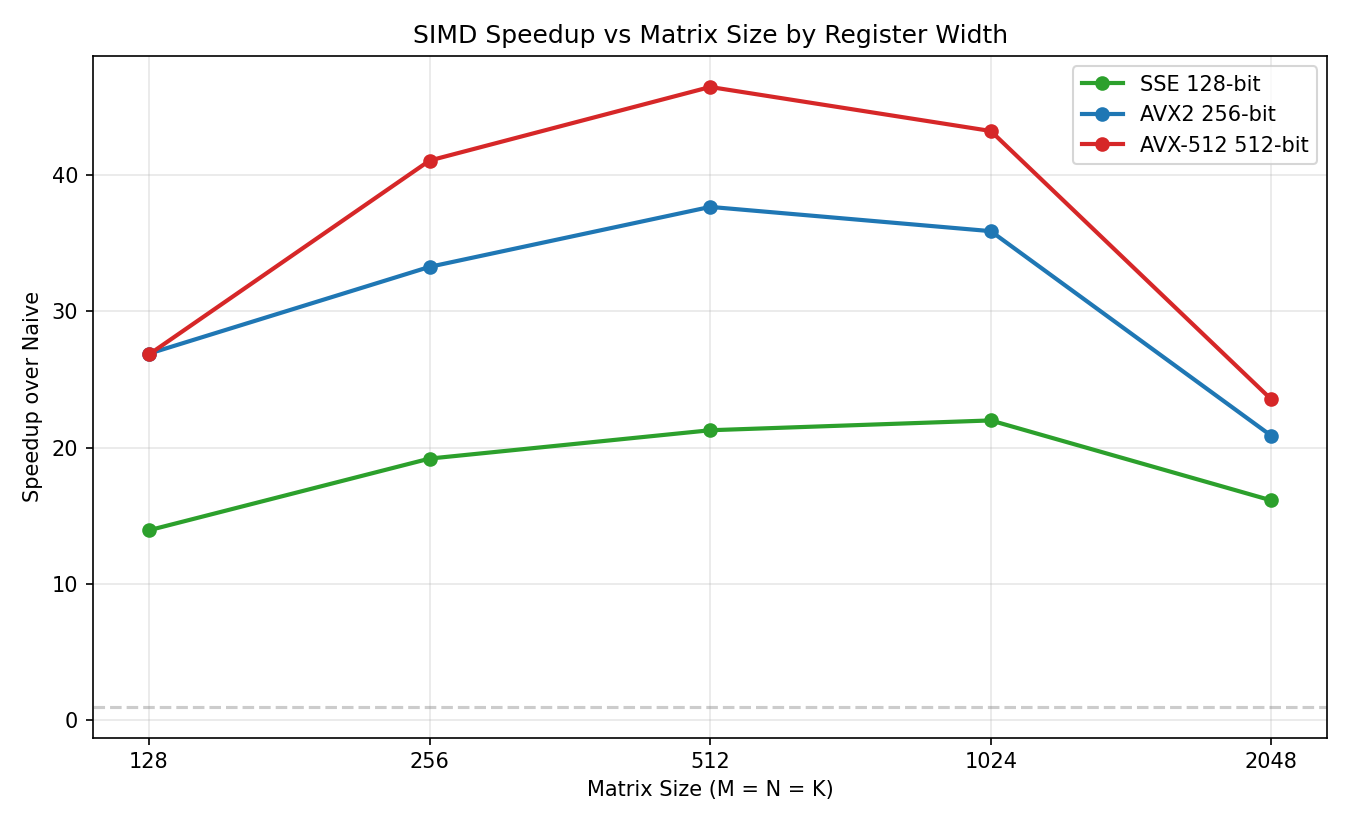
\includegraphics[width=0.8\textwidth]{../plots/simd_width_speedup.png}
\caption{SIMD speedup vs.\ matrix size for different register widths}
\end{figure}

\begin{figure}[H]
\centering
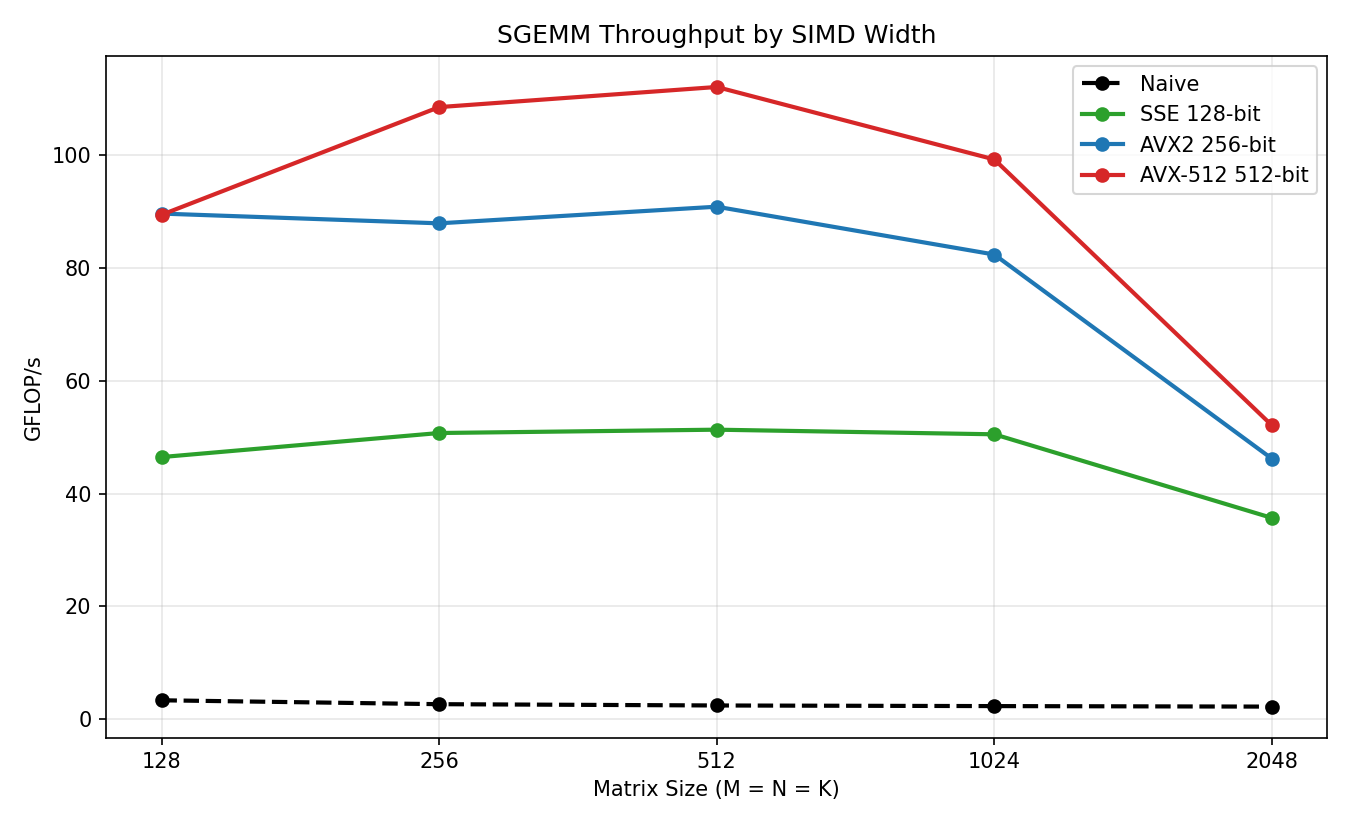
\includegraphics[width=0.8\textwidth]{../plots/simd_width_gflops.png}
\caption{SGEMM throughput (GFLOP/s) by SIMD width}
\end{figure}

\begin{figure}[H]
\centering
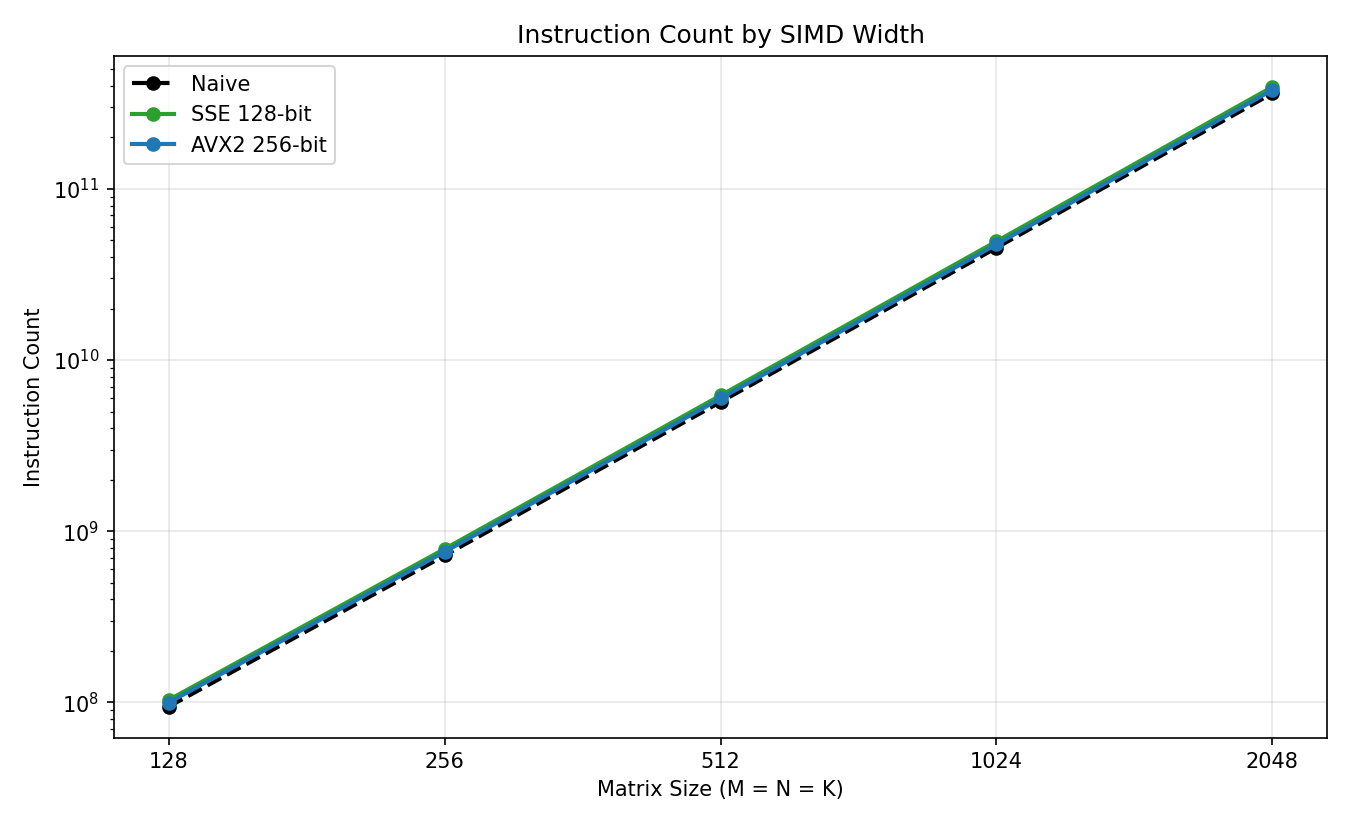
\includegraphics[width=0.8\textwidth]{../plots/simd_width_insns.png}
\caption{Instruction count by SIMD width (log scale)}
\end{figure}

\subsection{Analysis Questions}

\subsubsection{Q1: Speedup Trends}

Three trends are visible:

\begin{enumerate}
    \item \textbf{Wider SIMD $\Rightarrow$ higher peak speedup.}
    AVX-512 reaches \simdWidthAVXFiveTwelveFtwelveSpeedup{} at $512{\times}512$, AVX2 reaches \simdWidthAVXFtwelveSpeedup{}, and SSE reaches \simdWidthSSEFtwelveSpeedup{}.
    The ratio tracks the vector width (roughly $2{\times}$ per doubling) but falls short of the theoretical $4{\times}$/$8{\times}$/$16{\times}$ due to load/broadcast overhead and the horizontal reduction at the end.

    \item \textbf{Speedup rises then falls with matrix size.}
    At small sizes (128) the loop overhead and scalar cleanup dominate, limiting SSE to \simdWidthSSEOhtwentyeightSpeedup{}.
    Peak is around $512$--$1024$, where the working set fits mostly in L2 and the micro-kernel runs at near-peak throughput.
    At $2048$ all widths drop significantly (AVX-512 falls from \simdWidthAVXFiveTwelveFtwelveSpeedup{} to \simdWidthAVXFiveTwelveTfortyeightSpeedup{}) because the $A$ and $B$ matrices no longer fit in L2, and the unblocked kernel becomes memory-bound.

    \item \textbf{AVX2 and AVX-512 converge at small sizes.}
    At $128{\times}128$, AVX2 (\simdWidthAVXOhtwentyeightSpeedup{}) nearly matches AVX-512 (\simdWidthAVXFiveTwelveOhtwentyeightSpeedup{}) because the problem is too small for the wider vector to amortize its overhead.
\end{enumerate}

\subsubsection{Q2: Best SIMD Width}

\textbf{AVX-512 (512-bit)} achieves the maximum speedup at every matrix size where the kernel is not memory-bound.
The peak is \simdWidthAVXFiveTwelveFtwelveSpeedup{} at $512{\times}512$ (\simdWidthAVXFiveTwelveFtwelveGflops{} GFLOP/s).
This is expected: each 512-bit FMA processes 16 floats, double AVX2's 8, so the arithmetic throughput doubles while instruction-issue overhead stays roughly constant.

However, at $2048{\times}2048$ the advantage narrows (AVX-512 \simdWidthAVXFiveTwelveTfortyeightSpeedup{} vs AVX2 \simdWidthAVXTfortyeightSpeedup{}) because the bottleneck shifts from compute to memory bandwidth.
Cache blocking (Task 2C) is required to sustain AVX-512's higher throughput at large sizes.

% ============================================================================
\section{Task 2C: Software Prefetching + SIMD (3 points)}
% ============================================================================

\subsection{Combined Implementation}

The combined kernel (\texttt{matmul\_optimized.cpp}) layers three techniques on top of the Stage-1 SIMD micro-kernel:

\begin{enumerate}[nosep]
    \item \textbf{6$\times$16 AVX2 micro-kernel.} Each output tile spans 6 rows of $C$ and 16 contiguous columns, held in 12 \texttt{\_\_m256} accumulators (two per row: \texttt{c0l}/\texttt{c0h} through \texttt{c5l}/\texttt{c5h}).
    Per $K$ step: 2 packed-$B$ loads + 6 $A$ broadcasts $\rightarrow$ 12 FMAs.
    The 12 independent chains hide FMA latency and keep the pipeline saturated.

    \item \textbf{B-panel packing.} $B$ is stored column-major (K contiguous per column), so loading 16 columns at position $p$ would be strided.
    Before each $NC$-column block, $B$ is packed into a scratch buffer $\texttt{Bpack}[p][j]$ so that the micro-kernel's $B$ loads are unit-stride.

    \item \textbf{Cache blocking.} The output is traversed in $MC{\times}NC$ blocks (default $MC{=}96$, $NC{=}64$) with loop order $jc \rightarrow ic \rightarrow jr \rightarrow ir$.
    The packed $B$ panel ($K \times NC$ floats) is reused across all $MC$ rows, and each $A$ sub-panel ($MC \times K$) is reused across all $NC$ columns, so both stay resident in L2.
\end{enumerate}

\subsection{Software Prefetch in the Combined Kernel}

The combined kernel deliberately ships \emph{without} software prefetch. This was a
measured decision, not an omission. We added \texttt{\_mm\_prefetch} on the packed-$B$
stream (distance and fill level as compile-time knobs, default 64 floats ahead, T0) and
compared against the identical kernel without it, interleaved back-to-back on a pinned
core so thermal drift affects both variants equally
(variants preserved in \texttt{bench/experiments/}):

\begin{table}[H]
\centering
\caption{Software prefetch on the combined kernel, \texttt{optimized} stage, $1024^3$ (ms)}
\begin{tabular}{lrr}
\toprule
Variant & Times (interleaved) & Mean \\
\midrule
No prefetch                & 22.7 / 22.3 / 21.4 & $\sim$22.1 \\
$B$-stream prefetch        & 23.3 / 22.4 / 23.8 & $\sim$23.2 \\
$B$ + all six $A$ streams  & 26.2 -- 31.3       & $\sim$28 \\
\bottomrule
\end{tabular}
\end{table}

Prefetching is 0--5\% \emph{slower} on the $B$ stream and $\sim$25\% slower when the six
$A$ broadcast streams are prefetched as well. The mechanism: packing already converts
every inner-loop access into a unit-stride walk, which the L2 hardware streamer predicts
perfectly, so the software hint adds no information --- it only spends load-port slots
that the 12-FMA-per-8-load inner loop cannot spare. This is consistent with the flat
distance curve in the standalone prefetch stage (Task 2A).

\subsection{Software Prefetch on the Unblocked SIMD Kernel}

To confirm that this null result is a property of the \emph{blocked, packed} kernel and
not of software prefetch itself, we ran the same experiment on the Stage-1 SIMD kernel,
which has no cache blocking (prefetch on its two $B$ streams, 64 floats ahead, T0):

\begin{table}[H]
\centering
\caption{Prefetch on the unblocked SIMD kernel, \texttt{simd} stage times (ms), interleaved}
\begin{tabular}{lrrl}
\toprule
Size & Without & With & Verdict \\
\midrule
$128^3$  & 0.047--0.050 & 0.054--0.058 & $\sim$15\% slower \\
$256^3$  & 0.380        & 0.430--0.437 & $\sim$13\% slower \\
$512^3$  & 2.98--3.01   & 3.30--3.46   & $\sim$12\% slower \\
$1024^3$ & 26.3--26.6   & 28.3--29.5   & $\sim$9\% slower \\
$1536^3$ & 132.2 / 132.5 & 157.3 / 127.4 & wash (transition) \\
$2048^3$ & 366--464 (unstable) & \textbf{326--329 (stable)} & $\sim$20\% \textbf{faster} \\
\bottomrule
\end{tabular}
\end{table}

While the working set fits in cache, prefetch is pure overhead. Once it exceeds the L3
(at $2048^3$ three matrices total 48\,MB against a 12\,MB L3), demand misses reach DRAM,
the hardware prefetcher loses stream history under eviction pressure, and the constant
software lookahead genuinely hides latency --- $\sim$20\% faster \emph{and} the large
run-to-run variance collapses. Taken together, the two experiments say: \emph{software
prefetch is a substitute for locality, not an addition to it}. A kernel that already has
locality (blocking + packing) gains nothing at any size; a kernel that lacks it gains
exactly where the hardware gives up.

\todo{Both experiment tables above were measured on the i5-11400H; re-collect on the
machine the report standardises on (bench/experiments/README.md has the build commands;
the crossover size scales with that machine's L3 capacity).}

\subsection{Hardware Counter Analysis}

\todo{Hardware counter table and analysis to be updated after Task 2A prefetch code is finalized and perf counters are re-collected.}

\begin{table}[H]
\centering
\caption{Hardware counters per stage ($M{=}N{=}K{=}1024$, cold cache)}
\resizebox{\textwidth}{!}{%
\begin{tabular}{lrrrrr}
\toprule
Stage & Instructions & L1-D Misses & L2 Misses & LLC Misses & IPC \\
\midrule
Naive           & \perfNaiveInsns & \perfNaiveLoneDmiss & \perfNaiveLtwoMiss & \perfNaiveLLCmiss & \perfNaiveIPC \\
SIMD            & \perfSimdInsns & \perfSimdLoneDmiss & \perfSimdLtwoMiss & \perfSimdLLCmiss & \perfSimdIPC \\
Prefetch        & \todo{re-run} & \todo{re-run} & \todo{re-run} & \todo{re-run} & \todo{re-run} \\
Prefetch + SIMD & \perfOptimizedInsns & \perfOptimizedLoneDmiss & \perfOptimizedLtwoMiss & \perfOptimizedLLCmiss & \perfOptimizedIPC \\
\bottomrule
\end{tabular}%
}
\end{table}

\todo{Key observations to be rewritten once prefetch row is updated.}

\begin{figure}[H]
\centering
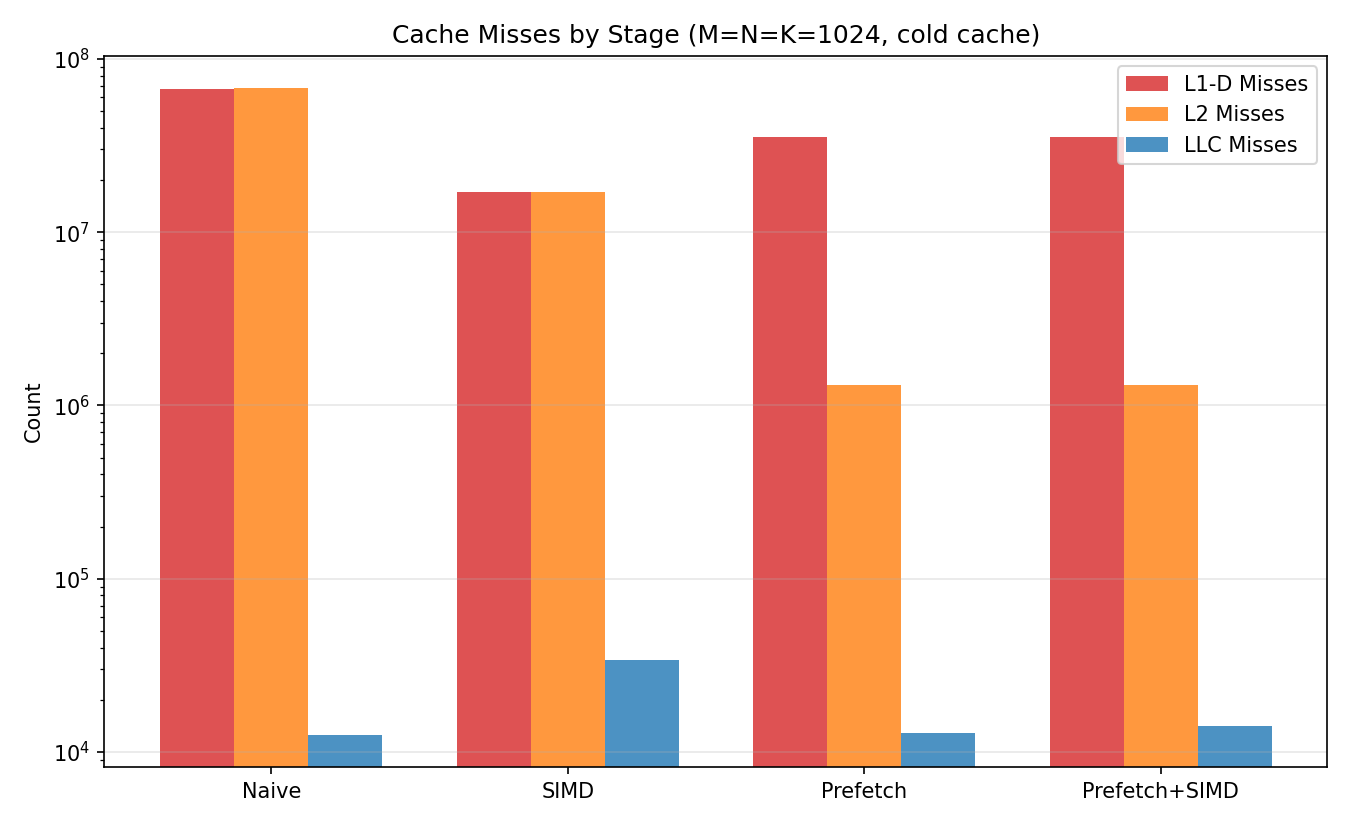
\includegraphics[width=0.8\textwidth]{../plots/perf_cache_misses.png}
\caption{Cache misses by stage (M=N=K=1024, cold cache, log scale). \todo{Regenerate after prefetch re-run.}}
\end{figure}

\begin{figure}[H]
\centering
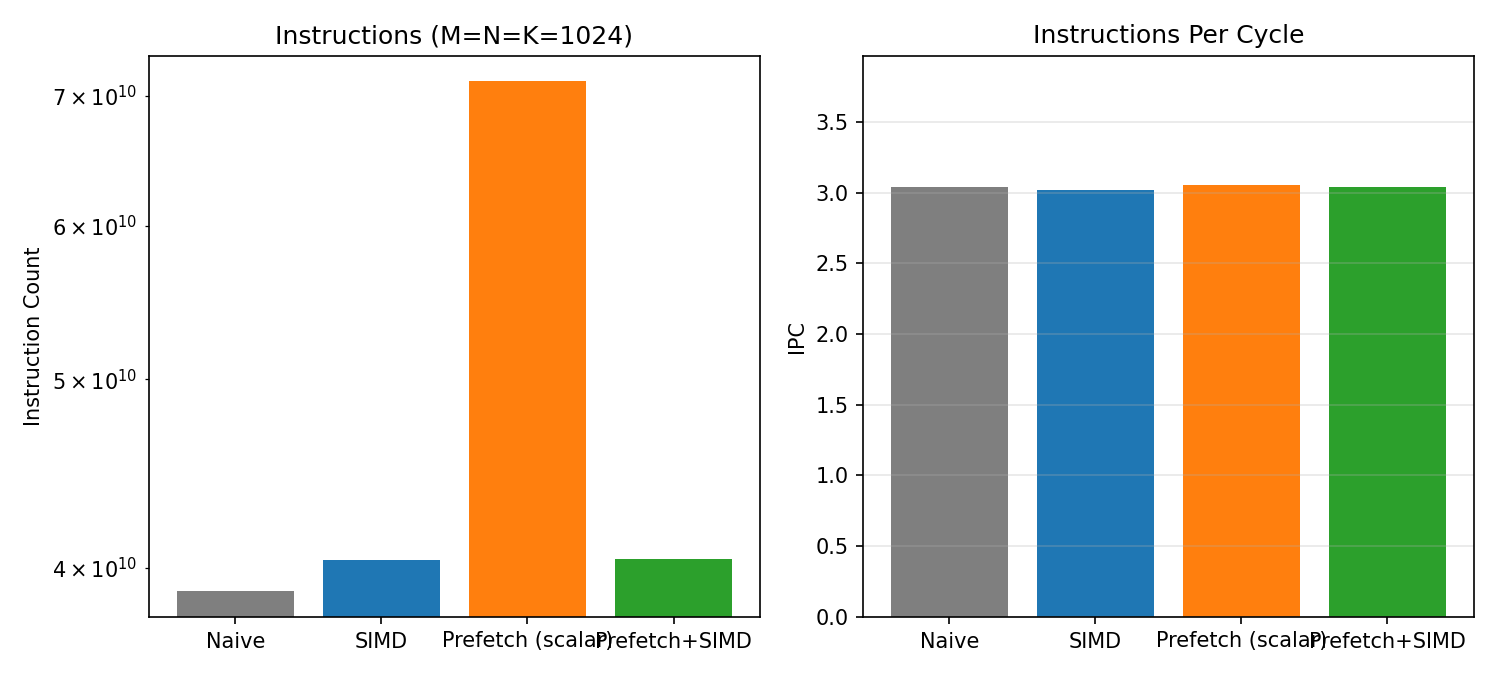
\includegraphics[width=0.8\textwidth]{../plots/perf_insns_ipc.png}
\caption{Instruction count and IPC by stage (M=N=K=1024). \todo{Regenerate after prefetch re-run.}}
\end{figure}

\subsection{Final Performance Summary}

\begin{figure}[H]
\centering
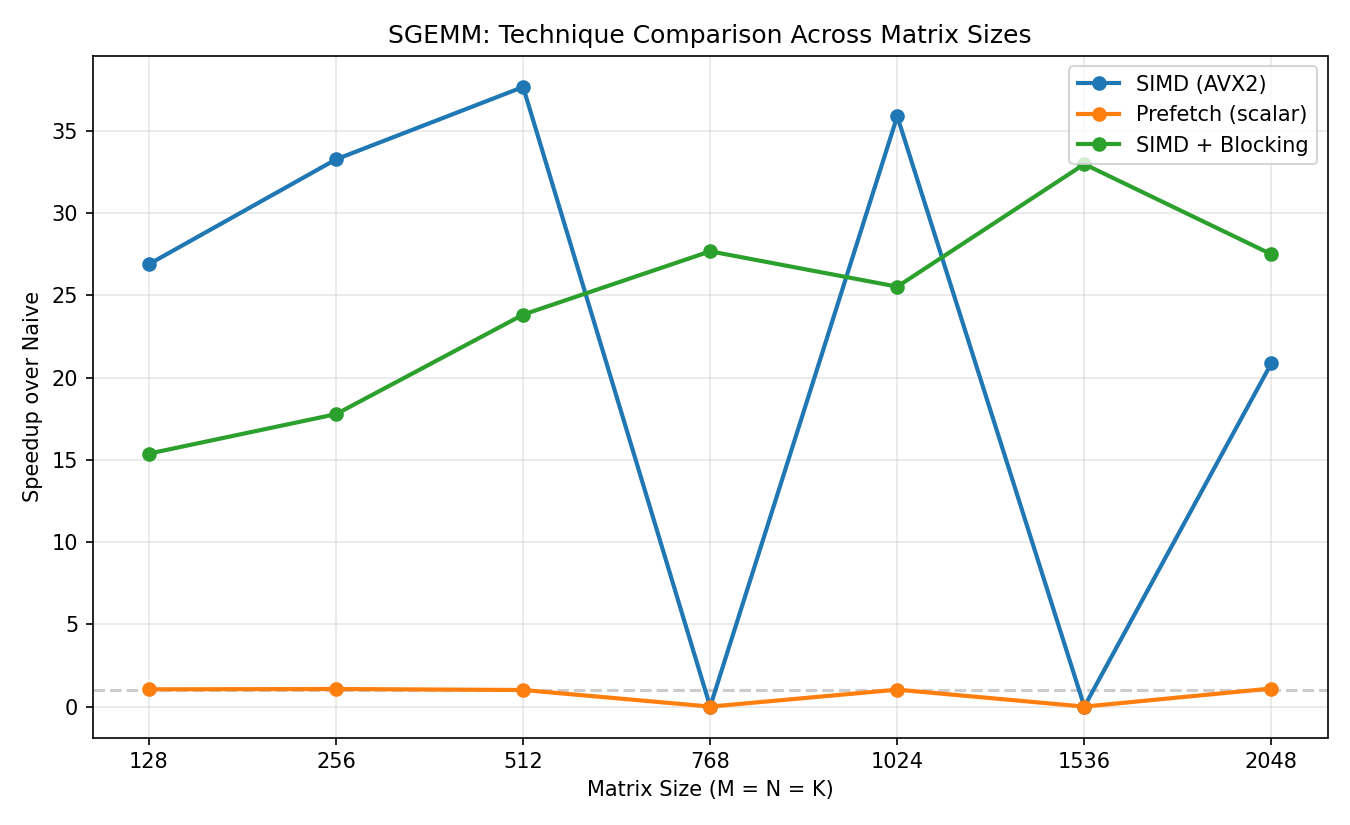
\includegraphics[width=0.85\textwidth]{../plots/task2_final_comparison.png}
\caption{Technique comparison across matrix sizes: speedup over naive SGEMM.}
\end{figure}

\begin{figure}[H]
\centering
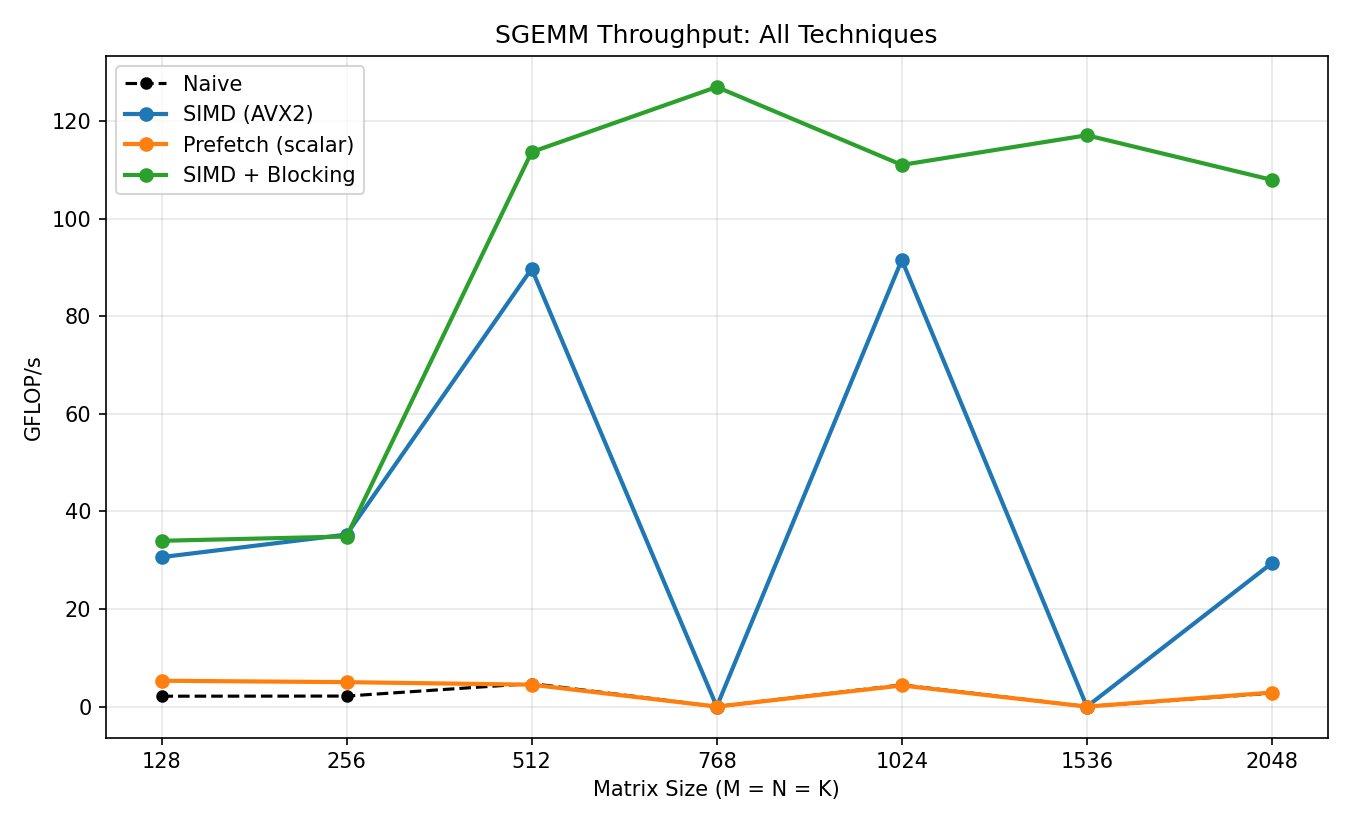
\includegraphics[width=0.85\textwidth]{../plots/task2_gflops_comparison.png}
\caption{SGEMM throughput (GFLOP/s) for all techniques.}
\end{figure}

\begin{table}[H]
\centering
\caption{Best speedup per technique across matrix sizes}
\begin{tabular}{lrrr}
\toprule
Matrix Size & SIMD & Prefetch & Prefetch + SIMD \\
\midrule
128   & \sweepSimdOhtwentyeightSpeedup & \todo{re-run} & \sweepOptimizedOhtwentyeightSpeedup \\
256   & \sweepSimdTwofiftysixSpeedup & \todo{re-run} & \sweepOptimizedTwofiftysixSpeedup \\
512   & \sweepSimdFtwelveSpeedup & \todo{re-run} & \sweepOptimizedFtwelveSpeedup \\
1024  & \sweepSimdTtwentyfourSpeedup & \todo{re-run} & \sweepOptimizedTtwentyfourSpeedup \\
2048  & \sweepSimdTfortyeightSpeedup & \todo{re-run} & \sweepOptimizedTfortyeightSpeedup \\
\bottomrule
\end{tabular}
\end{table}

\subsection{Analysis: Synergy Between Techniques}

\todo{Synergy analysis to be rewritten after Task 2A prefetch results are finalized. The key argument --- SIMD removes the compute bottleneck while blocking removes the memory bottleneck, and the combination exceeds either alone --- will remain, but the specific numbers (prefetch-only speedup, crossover point, GFLOP/s comparisons) need to come from the updated prefetch data.}

The combined kernel achieves a peak of \sweepOptimizedFifteenthirtysixSpeedup{} at $1536{\times}1536$.

The synergy is not additive but \emph{complementary}:
\begin{itemize}[nosep]
    \item \textbf{SIMD without blocking} is compute-efficient at small sizes but becomes memory-bound at large sizes. At $2048$, SIMD-only drops to \sweepSimdTfortyeightSpeedup{} because the operands spill out of L2 and every tile re-streams them from DRAM.

    \item \textbf{Blocking without SIMD} (the prefetch stage) keeps the data cache-resident but is limited by scalar instruction throughput. \todo{Update with actual prefetch-only throughput after 2A re-run.}

    \item \textbf{Combined}: cache blocking ensures the operands stay in L2, and SIMD ensures the FMA units are fully utilized while the data is resident. \todo{Update GFLOP/s comparisons and lift factors after 2A re-run.}

    \item The crossover point is clear in the speedup plot: SIMD-only dominates at small sizes (where data fits in cache anyway), but the combined kernel dominates at large sizes where blocking prevents the SIMD kernel from going memory-bound.
\end{itemize}

\end{document}
